% graph -> simplicial complex -> Hodge Laplacian L1 -> spectrum, in RWTH colours.
% Coordinates match public/research/scheme.svg (1 unit = 1pt, y pointing down).
\documentclass[tikz,border=4pt]{standalone}
\definecolor{rwthBlue}{HTML}{00549F}
\definecolor{rwthMagenta}{HTML}{E30066}
\definecolor{rwthTurq}{HTML}{0098A1}
\definecolor{rwthGreen}{HTML}{57AB27}
\definecolor{rwthOrange}{HTML}{F6A800}
\definecolor{rwthPetrol}{HTML}{006165}
\colorlet{gray}{black!46}
\usetikzlibrary{arrows.meta}
\begin{document}
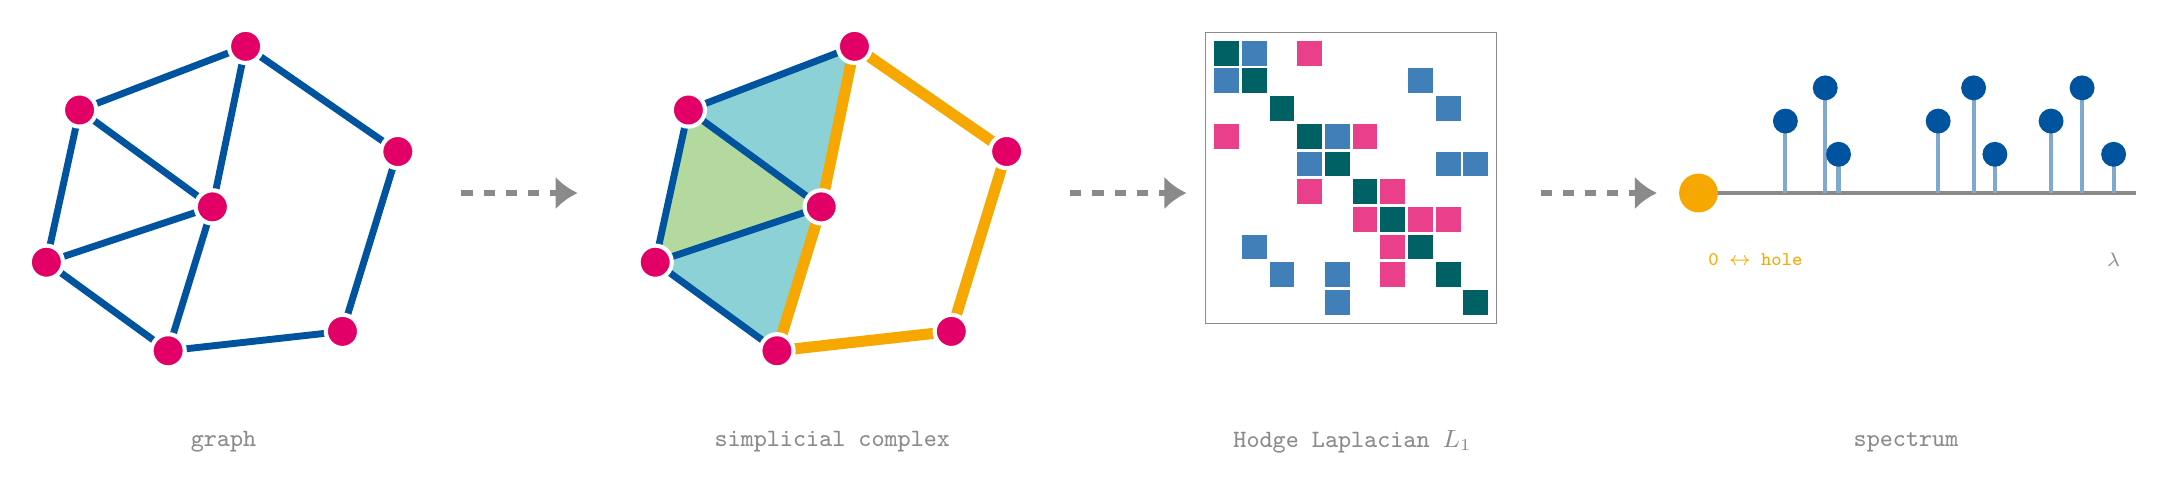
\begin{tikzpicture}[x=1pt,y=-1pt,
  edge/.style={rwthBlue,line width=2.5pt,line cap=round},
  hole/.style={rwthOrange,line width=4pt,line cap=round},
  vtx/.style={circle,fill=rwthMagenta,draw=white,line width=1.5pt,inner sep=0pt,minimum size=12pt},
  flow/.style={gray,line width=2pt,dash pattern=on 4pt off 4pt,-{Latex[length=8pt,width=12pt]}},
  lbl/.style={gray,font=\ttfamily\small}]
  % graph
  \draw[edge] (40,55) -- (100,32);
  \draw[edge] (40,55) -- (28,110);
  \draw[edge] (40,55) -- (88,90);
  \draw[edge] (100,32) -- (155,70);
  \draw[edge] (100,32) -- (88,90);
  \draw[edge] (155,70) -- (135,135);
  \draw[edge] (135,135) -- (72,142);
  \draw[edge] (72,142) -- (28,110);
  \draw[edge] (72,142) -- (88,90);
  \draw[edge] (28,110) -- (88,90);
  \foreach \p in {(40,55),(100,32),(155,70),(135,135),(72,142),(28,110),(88,90)} \node[vtx] at \p {};
  \node[lbl] at (92,175) {graph};
  \draw[flow] (178,85) -- ++(42,0);
  % simplicial complex, hole in orange
  \fill[rwthTurq,fill opacity=.45] (260,55) -- (320,32) -- (308,90) -- cycle;
  \fill[rwthGreen,fill opacity=.45] (260,55) -- (248,110) -- (308,90) -- cycle;
  \fill[rwthTurq,fill opacity=.45] (292,142) -- (248,110) -- (308,90) -- cycle;
  \draw[edge] (260,55) -- (320,32);
  \draw[edge] (260,55) -- (248,110);
  \draw[edge] (260,55) -- (308,90);
  \draw[hole] (320,32) -- (375,70);
  \draw[hole] (320,32) -- (308,90);
  \draw[hole] (375,70) -- (355,135);
  \draw[hole] (355,135) -- (292,142);
  \draw[edge] (292,142) -- (248,110);
  \draw[hole] (292,142) -- (308,90);
  \draw[edge] (248,110) -- (308,90);
  \foreach \p in {(260,55),(320,32),(375,70),(355,135),(292,142),(248,110),(308,90)} \node[vtx] at \p {};
  \node[lbl] at (312,175) {simplicial complex};
  \draw[flow] (398,85) -- ++(42,0);
  % Hodge Laplacian L1 = B1^T B1 + B2 B2^T (sparsity pattern)
  \fill[rwthPetrol] (450,30) rectangle ++(9,9);
  \fill[rwthBlue!75] (460,30) rectangle ++(9,9);
  \fill[rwthMagenta!75] (480,30) rectangle ++(9,9);
  \fill[rwthBlue!75] (450,40) rectangle ++(9,9);
  \fill[rwthPetrol] (460,40) rectangle ++(9,9);
  \fill[rwthBlue!75] (520,40) rectangle ++(9,9);
  \fill[rwthPetrol] (470,50) rectangle ++(9,9);
  \fill[rwthBlue!75] (530,50) rectangle ++(9,9);
  \fill[rwthMagenta!75] (450,60) rectangle ++(9,9);
  \fill[rwthPetrol] (480,60) rectangle ++(9,9);
  \fill[rwthBlue!75] (490,60) rectangle ++(9,9);
  \fill[rwthMagenta!75] (500,60) rectangle ++(9,9);
  \fill[rwthBlue!75] (480,70) rectangle ++(9,9);
  \fill[rwthPetrol] (490,70) rectangle ++(9,9);
  \fill[rwthBlue!75] (530,70) rectangle ++(9,9);
  \fill[rwthBlue!75] (540,70) rectangle ++(9,9);
  \fill[rwthMagenta!75] (480,80) rectangle ++(9,9);
  \fill[rwthPetrol] (500,80) rectangle ++(9,9);
  \fill[rwthMagenta!75] (510,80) rectangle ++(9,9);
  \fill[rwthMagenta!75] (500,90) rectangle ++(9,9);
  \fill[rwthPetrol] (510,90) rectangle ++(9,9);
  \fill[rwthMagenta!75] (520,90) rectangle ++(9,9);
  \fill[rwthMagenta!75] (530,90) rectangle ++(9,9);
  \fill[rwthBlue!75] (460,100) rectangle ++(9,9);
  \fill[rwthMagenta!75] (510,100) rectangle ++(9,9);
  \fill[rwthPetrol] (520,100) rectangle ++(9,9);
  \fill[rwthBlue!75] (470,110) rectangle ++(9,9);
  \fill[rwthBlue!75] (490,110) rectangle ++(9,9);
  \fill[rwthMagenta!75] (510,110) rectangle ++(9,9);
  \fill[rwthPetrol] (530,110) rectangle ++(9,9);
  \fill[rwthBlue!75] (490,120) rectangle ++(9,9);
  \fill[rwthPetrol] (540,120) rectangle ++(9,9);
  \draw[gray] (447,27) rectangle ++(105,105);
  \node[lbl] at (500,175) {Hodge Laplacian $L_1$};
  \draw[flow] (568,85) -- ++(42,0);
  % spectrum of L1
  \draw[gray,line width=1.5pt] (625,85) -- (783,85);
  \fill[rwthOrange] (625.0,85) circle (7);
  \draw[rwthBlue!50,line width=1.5pt] (656.4,85) -- (656.4,59); \fill[rwthBlue] (656.4,59) circle (4.5);
  \draw[rwthBlue!50,line width=1.5pt] (670.8,85) -- (670.8,47); \fill[rwthBlue] (670.8,47) circle (4.5);
  \draw[rwthBlue!50,line width=1.5pt] (675.6,85) -- (675.6,71); \fill[rwthBlue] (675.6,71) circle (4.5);
  \draw[rwthBlue!50,line width=1.5pt] (711.6,85) -- (711.6,59); \fill[rwthBlue] (711.6,59) circle (4.5);
  \draw[rwthBlue!50,line width=1.5pt] (724.4,85) -- (724.4,47); \fill[rwthBlue] (724.4,47) circle (4.5);
  \draw[rwthBlue!50,line width=1.5pt] (732.1,85) -- (732.1,71); \fill[rwthBlue] (732.1,71) circle (4.5);
  \draw[rwthBlue!50,line width=1.5pt] (752.4,85) -- (752.4,59); \fill[rwthBlue] (752.4,59) circle (4.5);
  \draw[rwthBlue!50,line width=1.5pt] (763.6,85) -- (763.6,47); \fill[rwthBlue] (763.6,47) circle (4.5);
  \draw[rwthBlue!50,line width=1.5pt] (775.0,85) -- (775.0,71); \fill[rwthBlue] (775.0,71) circle (4.5);
  \node[lbl,rwthOrange,anchor=west,font=\ttfamily\scriptsize] at (625,109) {0 $\leftrightarrow$ hole};
  \node[lbl,font=\ttfamily\scriptsize] at (775,109) {$\lambda$};
  \node[lbl] at (700.0,175) {spectrum};
\end{tikzpicture}
\end{document}
